\documentclass{article}
\usepackage{amsmath, fullpage}
\usepackage{adjustbox}
\usepackage{algorithm}
\usepackage{algorithmic}
\usepackage{cancel}
\usepackage{graphicx}
\usepackage{subcaption}
\usepackage{xcolor}
\usepackage{hyperref}
\usepackage{enumitem}
\usepackage{blkarray}
\usepackage{enumitem}
\usepackage{float}
\usepackage{biblatex}
\addbibresource{references.bib}
\usepackage{pdfpages}

% \def\zz{\par\zzz}
% \def\zzz#1{%
%  \ifx!#1\hfill\else
%  \makebox[.75em]{\ifx.#1\else\ifx|#1$|$\else#1\fi\fi}%
%  \expandafter\zzz
%  \fi}

\begin{document}

\title{PH 821 Course Project \\ Detecting a simulated gravitational-wave signal}
\author{Dhananjay Raman \\ 210050044}
\date{November 25, 2024}
\maketitle
% make table of contents
\tableofcontents
\section{Abstract}
Gravitational wave detection has revolutionized our understanding of the cosmos, offering a unique probe into compact binary mergers such as binary black hole (BBH), neutron star-black hole (NSBH), and binary neutron star (BNS) mergers. This study details the implementation of a pipeline to identify and analyze simulated gravitational wave signals using the PyCBC toolkit. The signal was sourced from a simulated strain data file, processed through various steps including high-pass filtering, whitening, and power spectral density estimation to enhance signal clarity.

A coarse-to-fine grid search was conducted in the mass parameter space (10-100 $M_\odot$), leveraging matched filtering techniques to identify the optimal masses of the binary black hole system. The resulting signal exhibited a strong signal-to-noise ratio (SNR), with a peak observed at $M_1 = 10.1 M_\odot$ and $M_2 = 9.4 M_\odot$ (values based on results). A template waveform aligned with the detected signal was used to compute the residual data by subtracting the template from the conditioned signal. The time-frequency characteristics of the original and subtracted data were compared to confirm the successful detection and subtraction of the gravitational wave signal.

This pipeline demonstrates the power of matched filtering in detecting weak astrophysical signals buried in noise and provides a robust framework for parameter estimation of compact binary mergers. Future extensions of this analysis could include exploring other higher-order waveform models and expanding the parameter space to include spins and eccentricity.

All the code used in this analysis is available in the appendix and on \href{https://github.com/DhanoHacks/PH821-Project-Detecting-GWs}{GitHub}.

\section{Methods}

This analysis was performed using the PyCBC library, a Python package tailored for gravitational wave data analysis. The methods employed in this analysis were adapted from publicly available tutorials on gravitational wave data analysis \cite{pycbc_tutorial, odw2020_tutorial}.

\subsection{Data Preprocessing}
The strain data from the Virgo detector was read from a .gwf file. To improve the data quality:
\begin{itemize}
    \item Low-frequency content was removed using a high-pass filter with a cutoff of 50 Hz.
    \item The data was downsampled to a uniform sampling rate of 2048 Hz.
    \item The first and last 2 seconds of the data were cropped to mitigate edge effects.
\end{itemize}

\subsection{Power Spectral Density (PSD) Estimation}
The PSD of the data was estimated using the Welch method over 4-second segments. The PSD was then interpolated to match the data's frequency resolution and truncated using the inverse spectrum truncation method to prevent noise amplification.

\subsection{Whitening and Bandpassing}
The strain data was whitened by dividing its Fourier transform by the square root of the PSD. Subsequently, the whitened data was bandpassed between 50 Hz and 512 Hz to isolate the relevant frequency range of the signal.

\subsection{Time-Frequency Analysis}
A Q-transform was applied to the whitened data to generate a time-frequency representation, which highlights transient features. Specific time and frequency windows were zoomed to focus on the merger signal.

\subsection{Matched Filtering}
Matched filtering was employed to search for compact binary coalescence signals (assuming non-spinning binary black holes) in the data. The following steps were performed:
\begin{itemize}
    \item A coarse grid of masses was explored using the SEOBNRv4 waveform approximant.
    \item The signal-to-noise ratio (SNR) was computed for each template, and the highest SNR was identified to determine the most likely binary parameters.
    \item A finer grid of masses based on the best pair of masses from the coarse search refined the parameter estimation.
\end{itemize}

\subsection{Template Generation and Signal Alignment}
The optimal waveform template was generated using the SEOBNRv4 approximant. The template was aligned with the data using the peak SNR time and scaled to match the detected amplitude and phase.

\subsection{Signal Subtraction}
The aligned template was subtracted from the conditioned data to evaluate the residual signal. The time-frequency representations of the original and subtracted data were compared to assess the effectiveness of the subtraction.

\section{Results}

\begin{figure}[H]
    \centering
    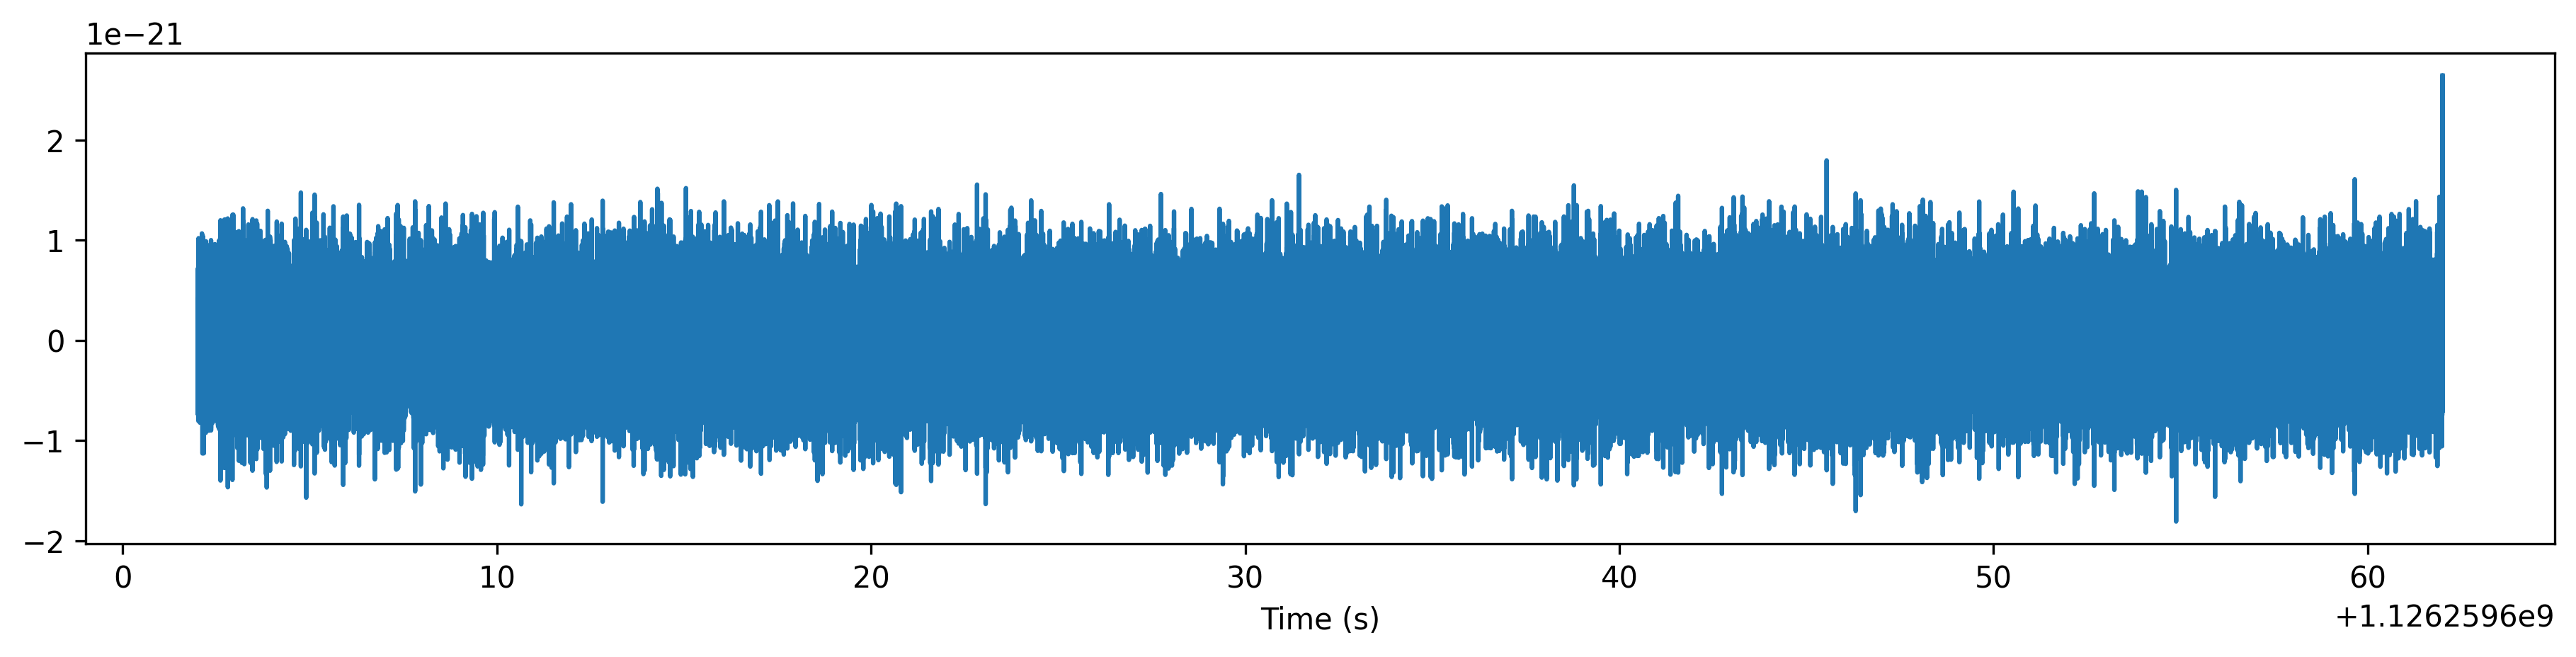
\includegraphics[width=\textwidth]{../plots/highpass_strain.png}
    \caption{High-pass filtered strain data. The low-frequency noise has been removed.}
    \label{fig:highpass_strain}
\end{figure}

\begin{figure}[H]
    \centering
    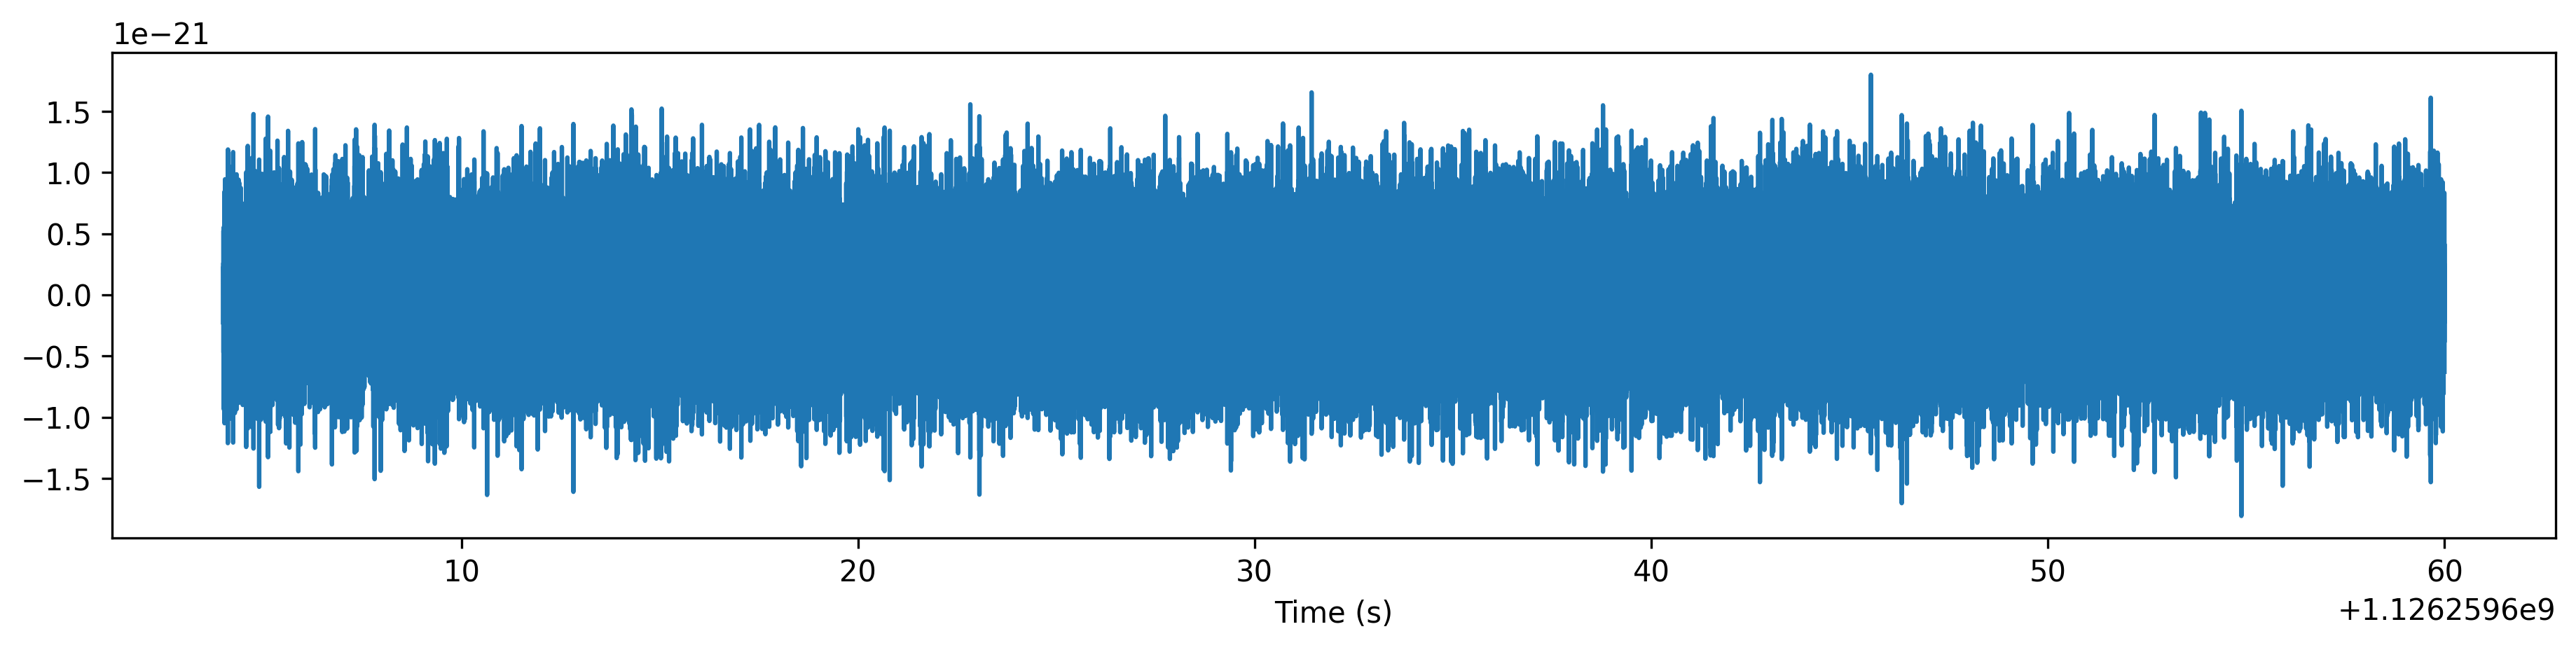
\includegraphics[width=\textwidth]{../plots/cropped_strain.png}
    \caption{High-pass filtered and cropped strain data. The low-frequency noise has been removed, and the data is cropped to remove edge effects.}
    \label{fig:cropped_strain}
\end{figure}

\begin{figure}[H]
    \centering
    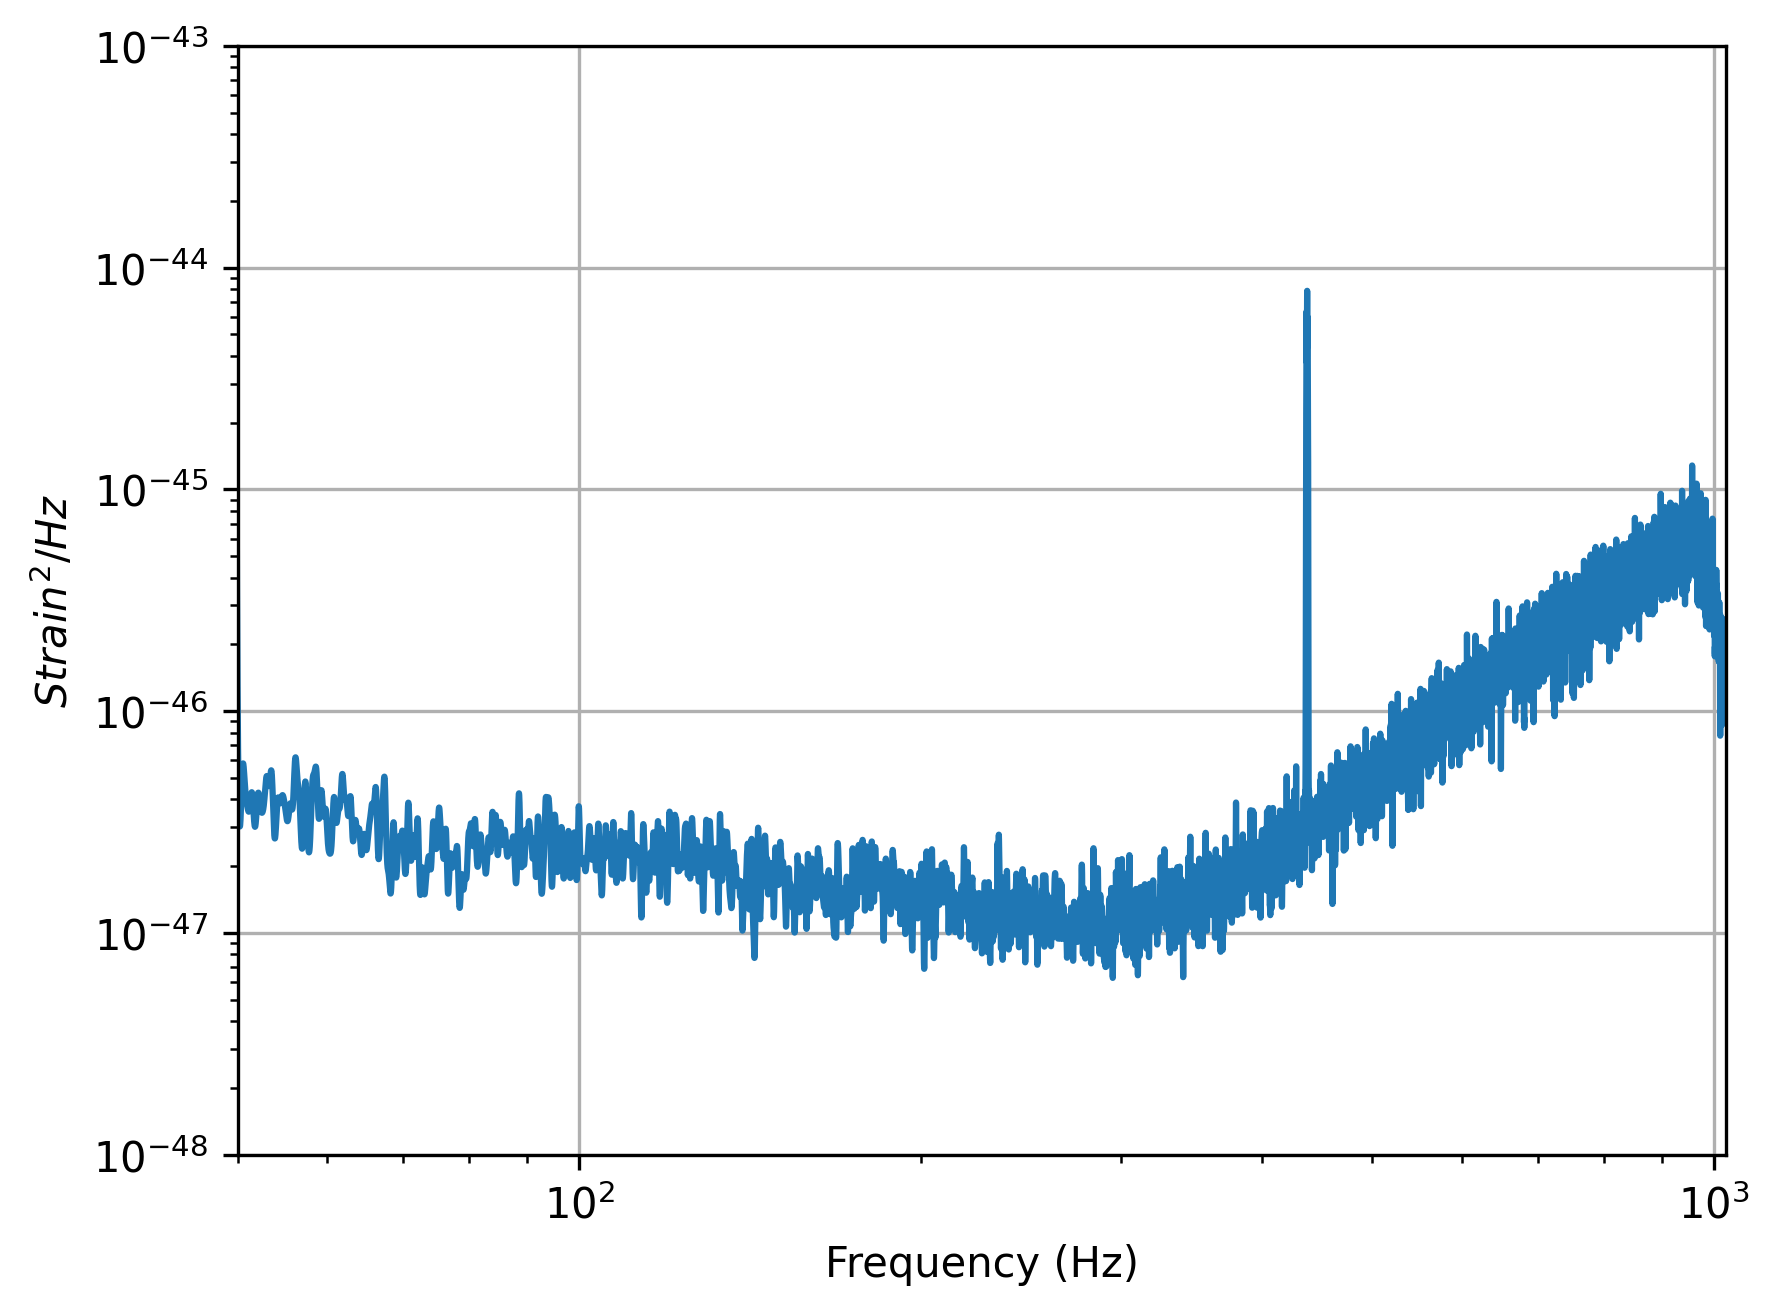
\includegraphics[width=\textwidth]{../plots/psd.png}
    \caption{Power spectral density of the High-pass filtered and cropped strain. The lower cutoff frequency was chosen as 50 Hz since the GW signal is weak below this frequency.}
    \label{fig:psd}
\end{figure}

\begin{figure}[H]
    \centering
    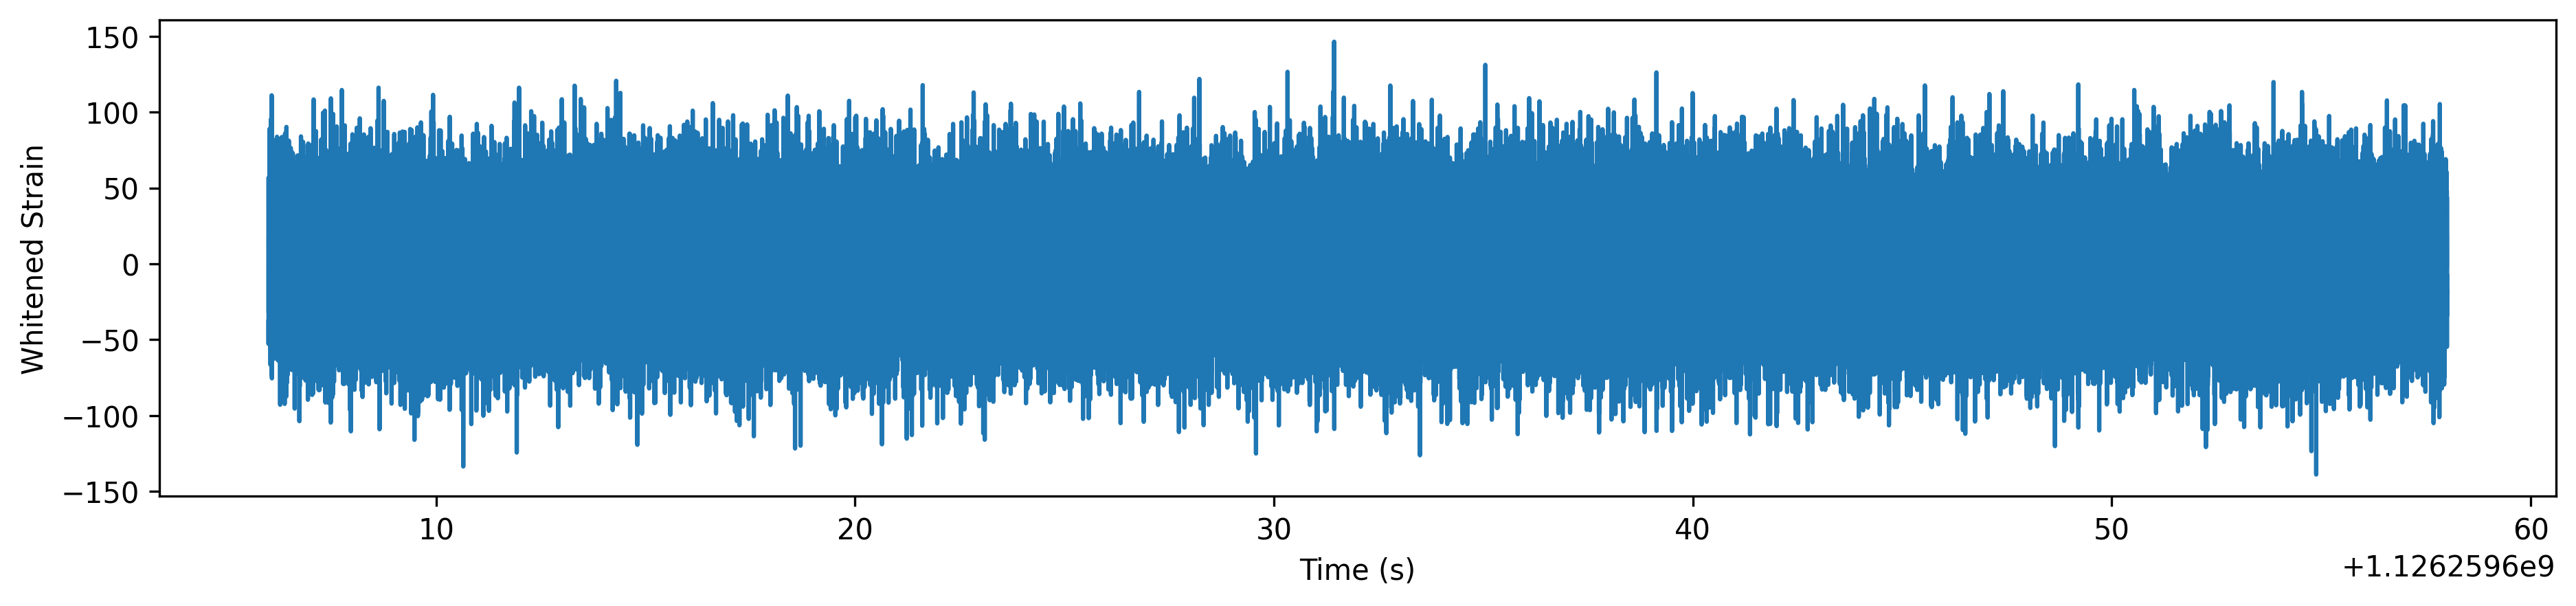
\includegraphics[width=\textwidth]{../plots/whitened_strain.png}
    \caption{Whitened strain data. Whitening enhances the signal by removing the frequency-dependent noise.}
    \label{fig:whitened_strain}
\end{figure}

\begin{figure}[H]
    \centering
    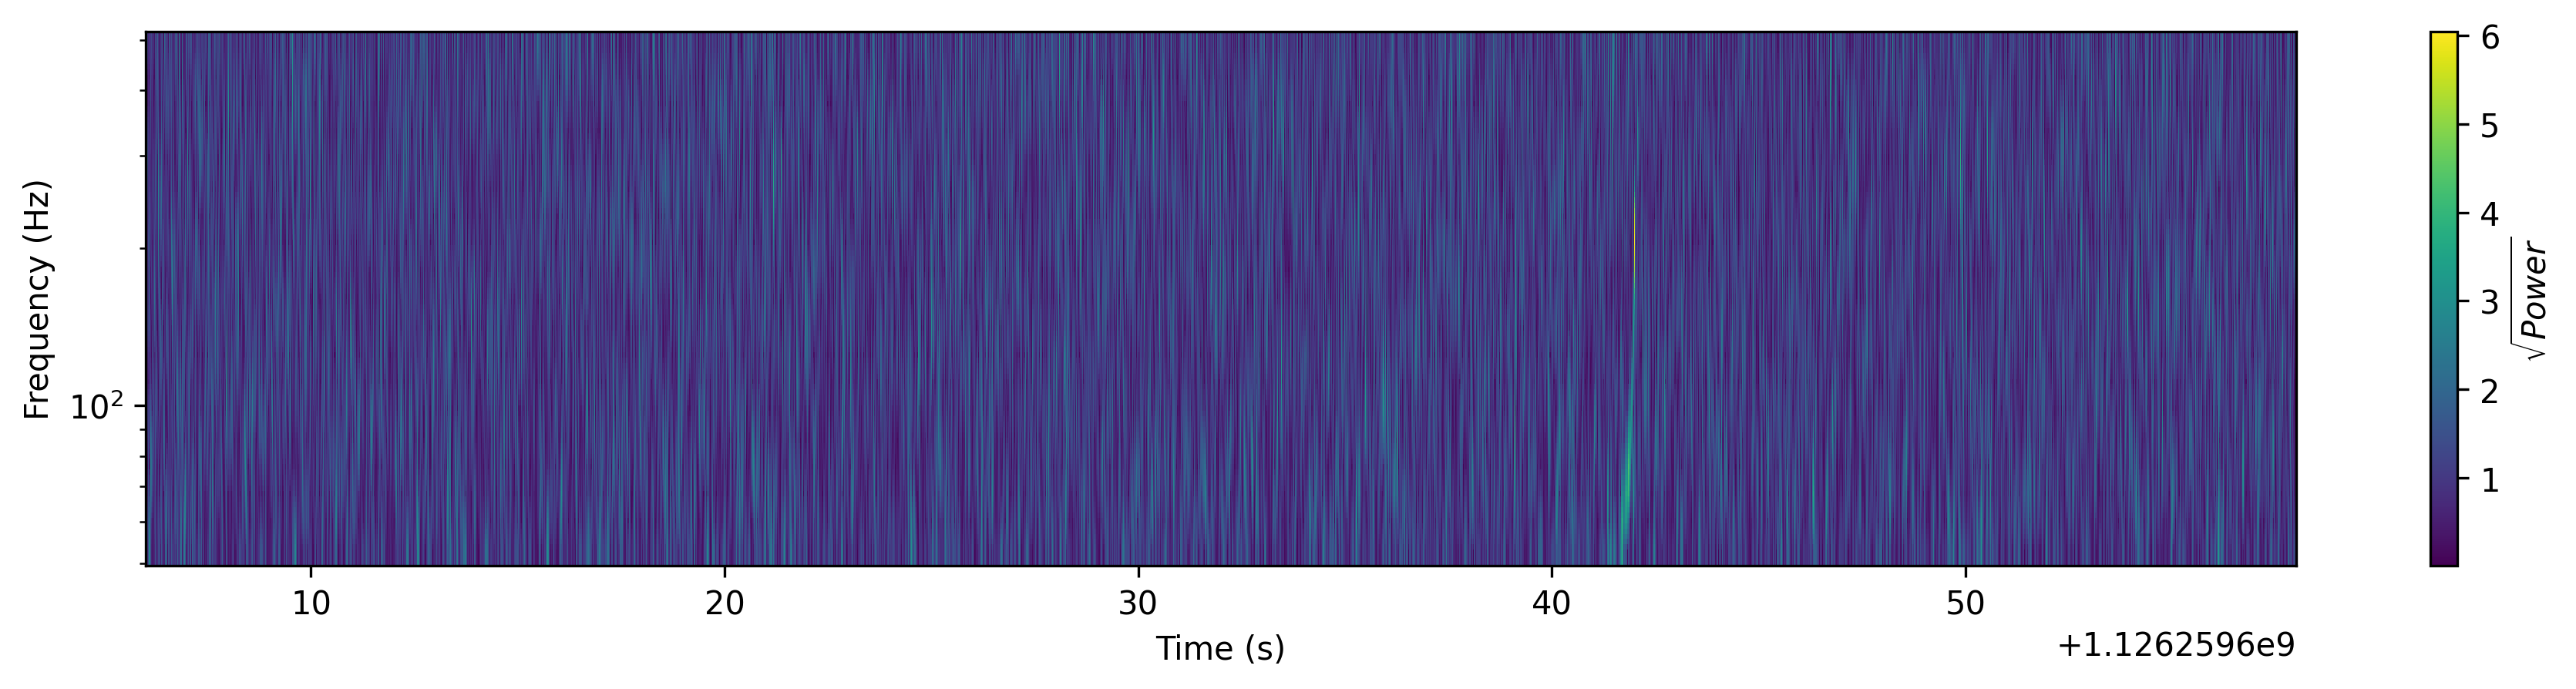
\includegraphics[width=\textwidth]{../plots/qtransform.png}
    \caption{Q-transform of the whitened data, showing the signal in time-frequency space. A transient feature is visible in the 50--300 Hz range.}
    \label{fig:qtransform}
\end{figure}

\begin{figure}[H]
    \centering
    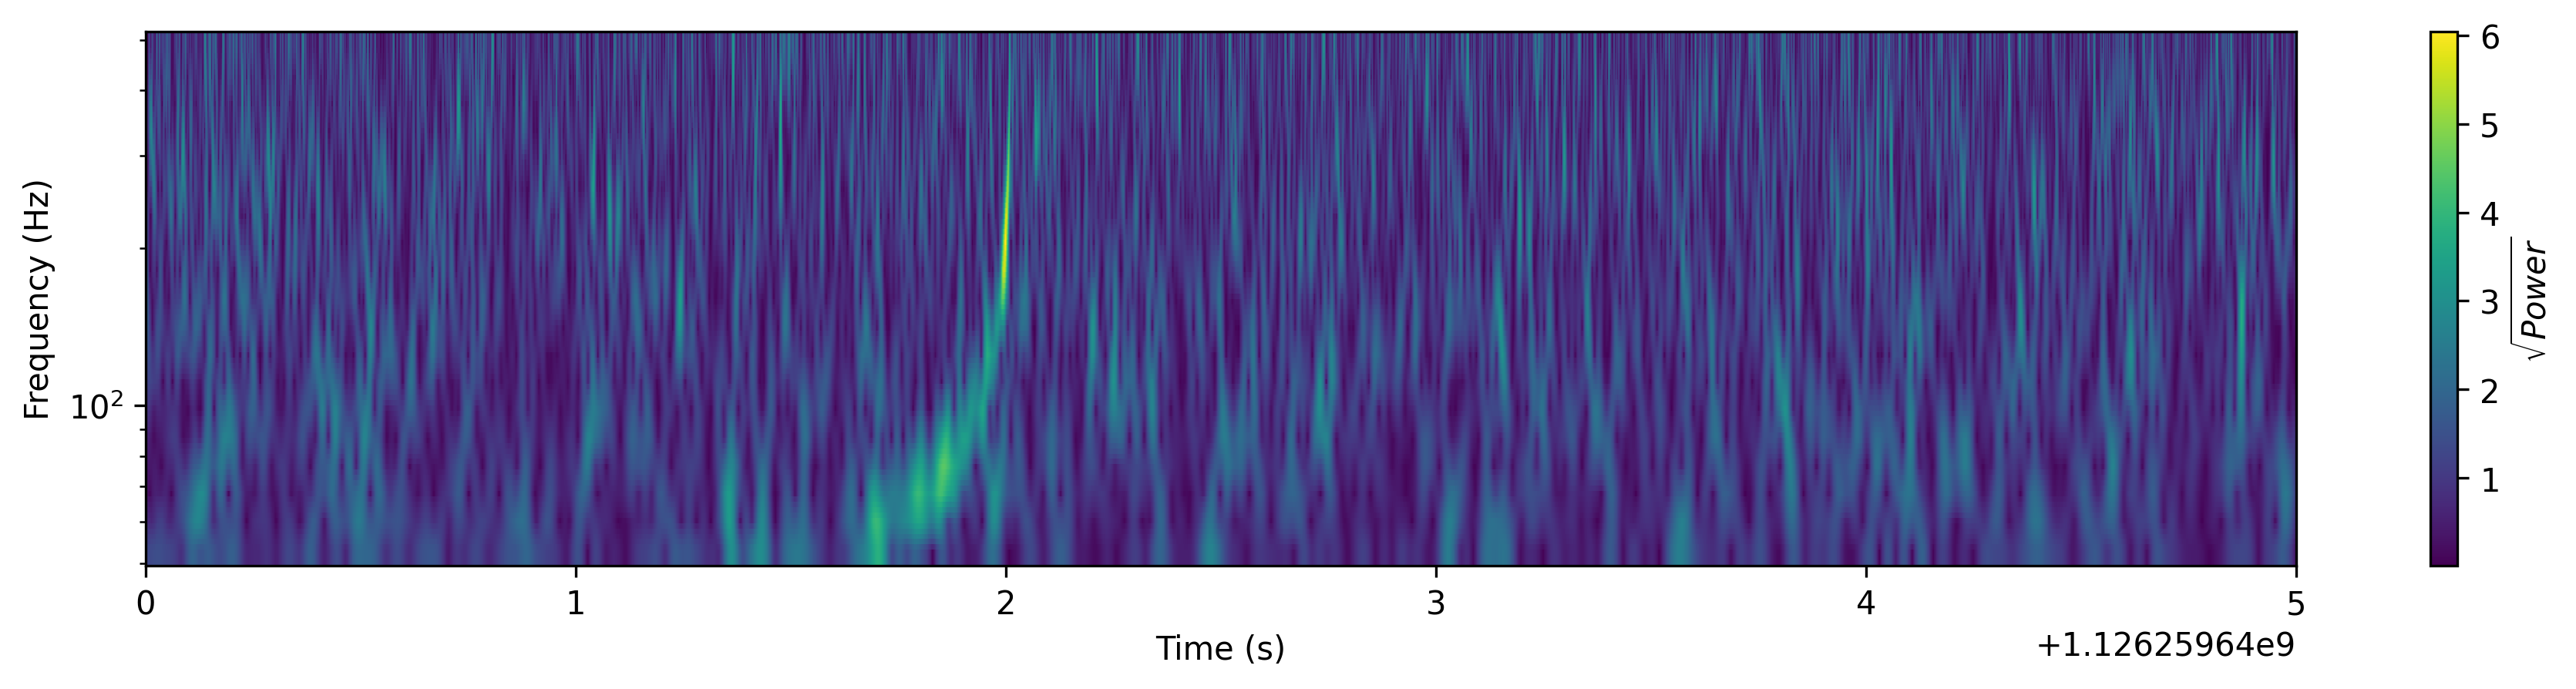
\includegraphics[width=\textwidth]{../plots/qtransform_zoomed.png}
    \caption{Zoomed Q-transform plot focusing on the signal around the merger time. The feature becomes more prominent in this view.}
    \label{fig:qtransform_zoomed}
\end{figure}

\begin{figure}[H]
    \centering
    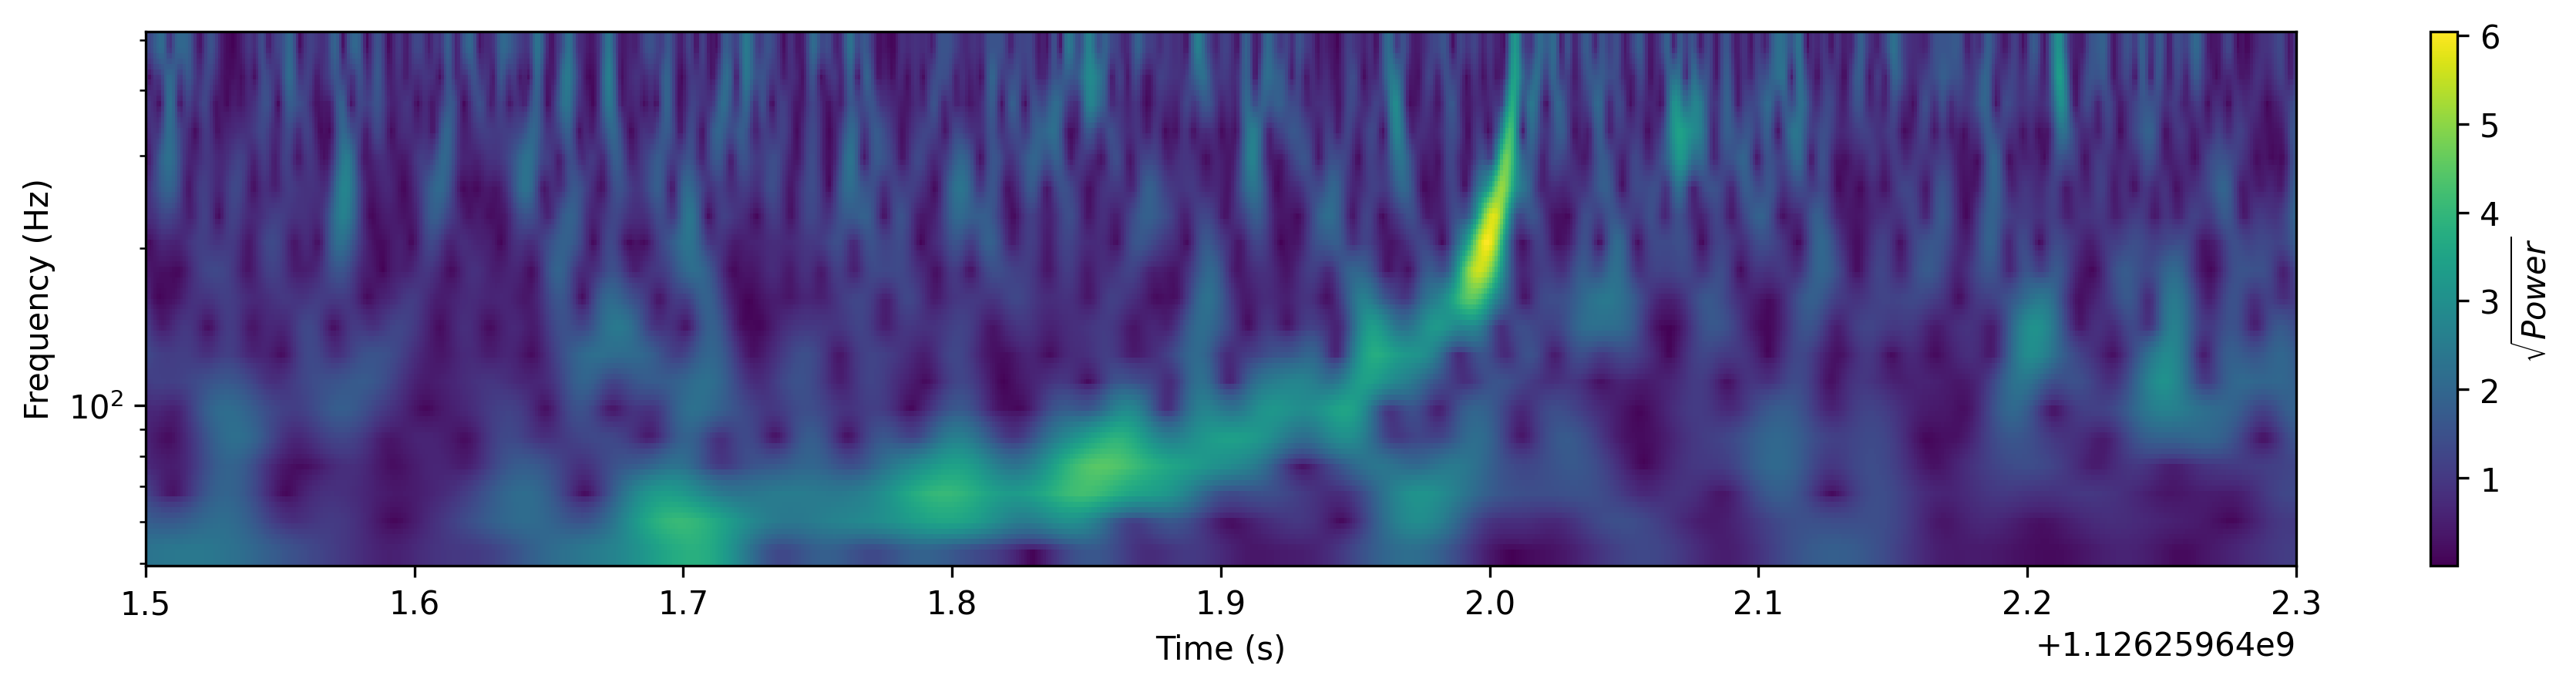
\includegraphics[width=\textwidth]{../plots/qtransform_zoomed2.png}
    \caption{Further zoomed Q-transform plot around the merger time. The signal is clearly visible in the time-frequency representation, with a coalescence time around 1126259642.0 seconds.}
    \label{fig:qtransform_zoomed2}
\end{figure}

\begin{figure}[H]
    \centering
    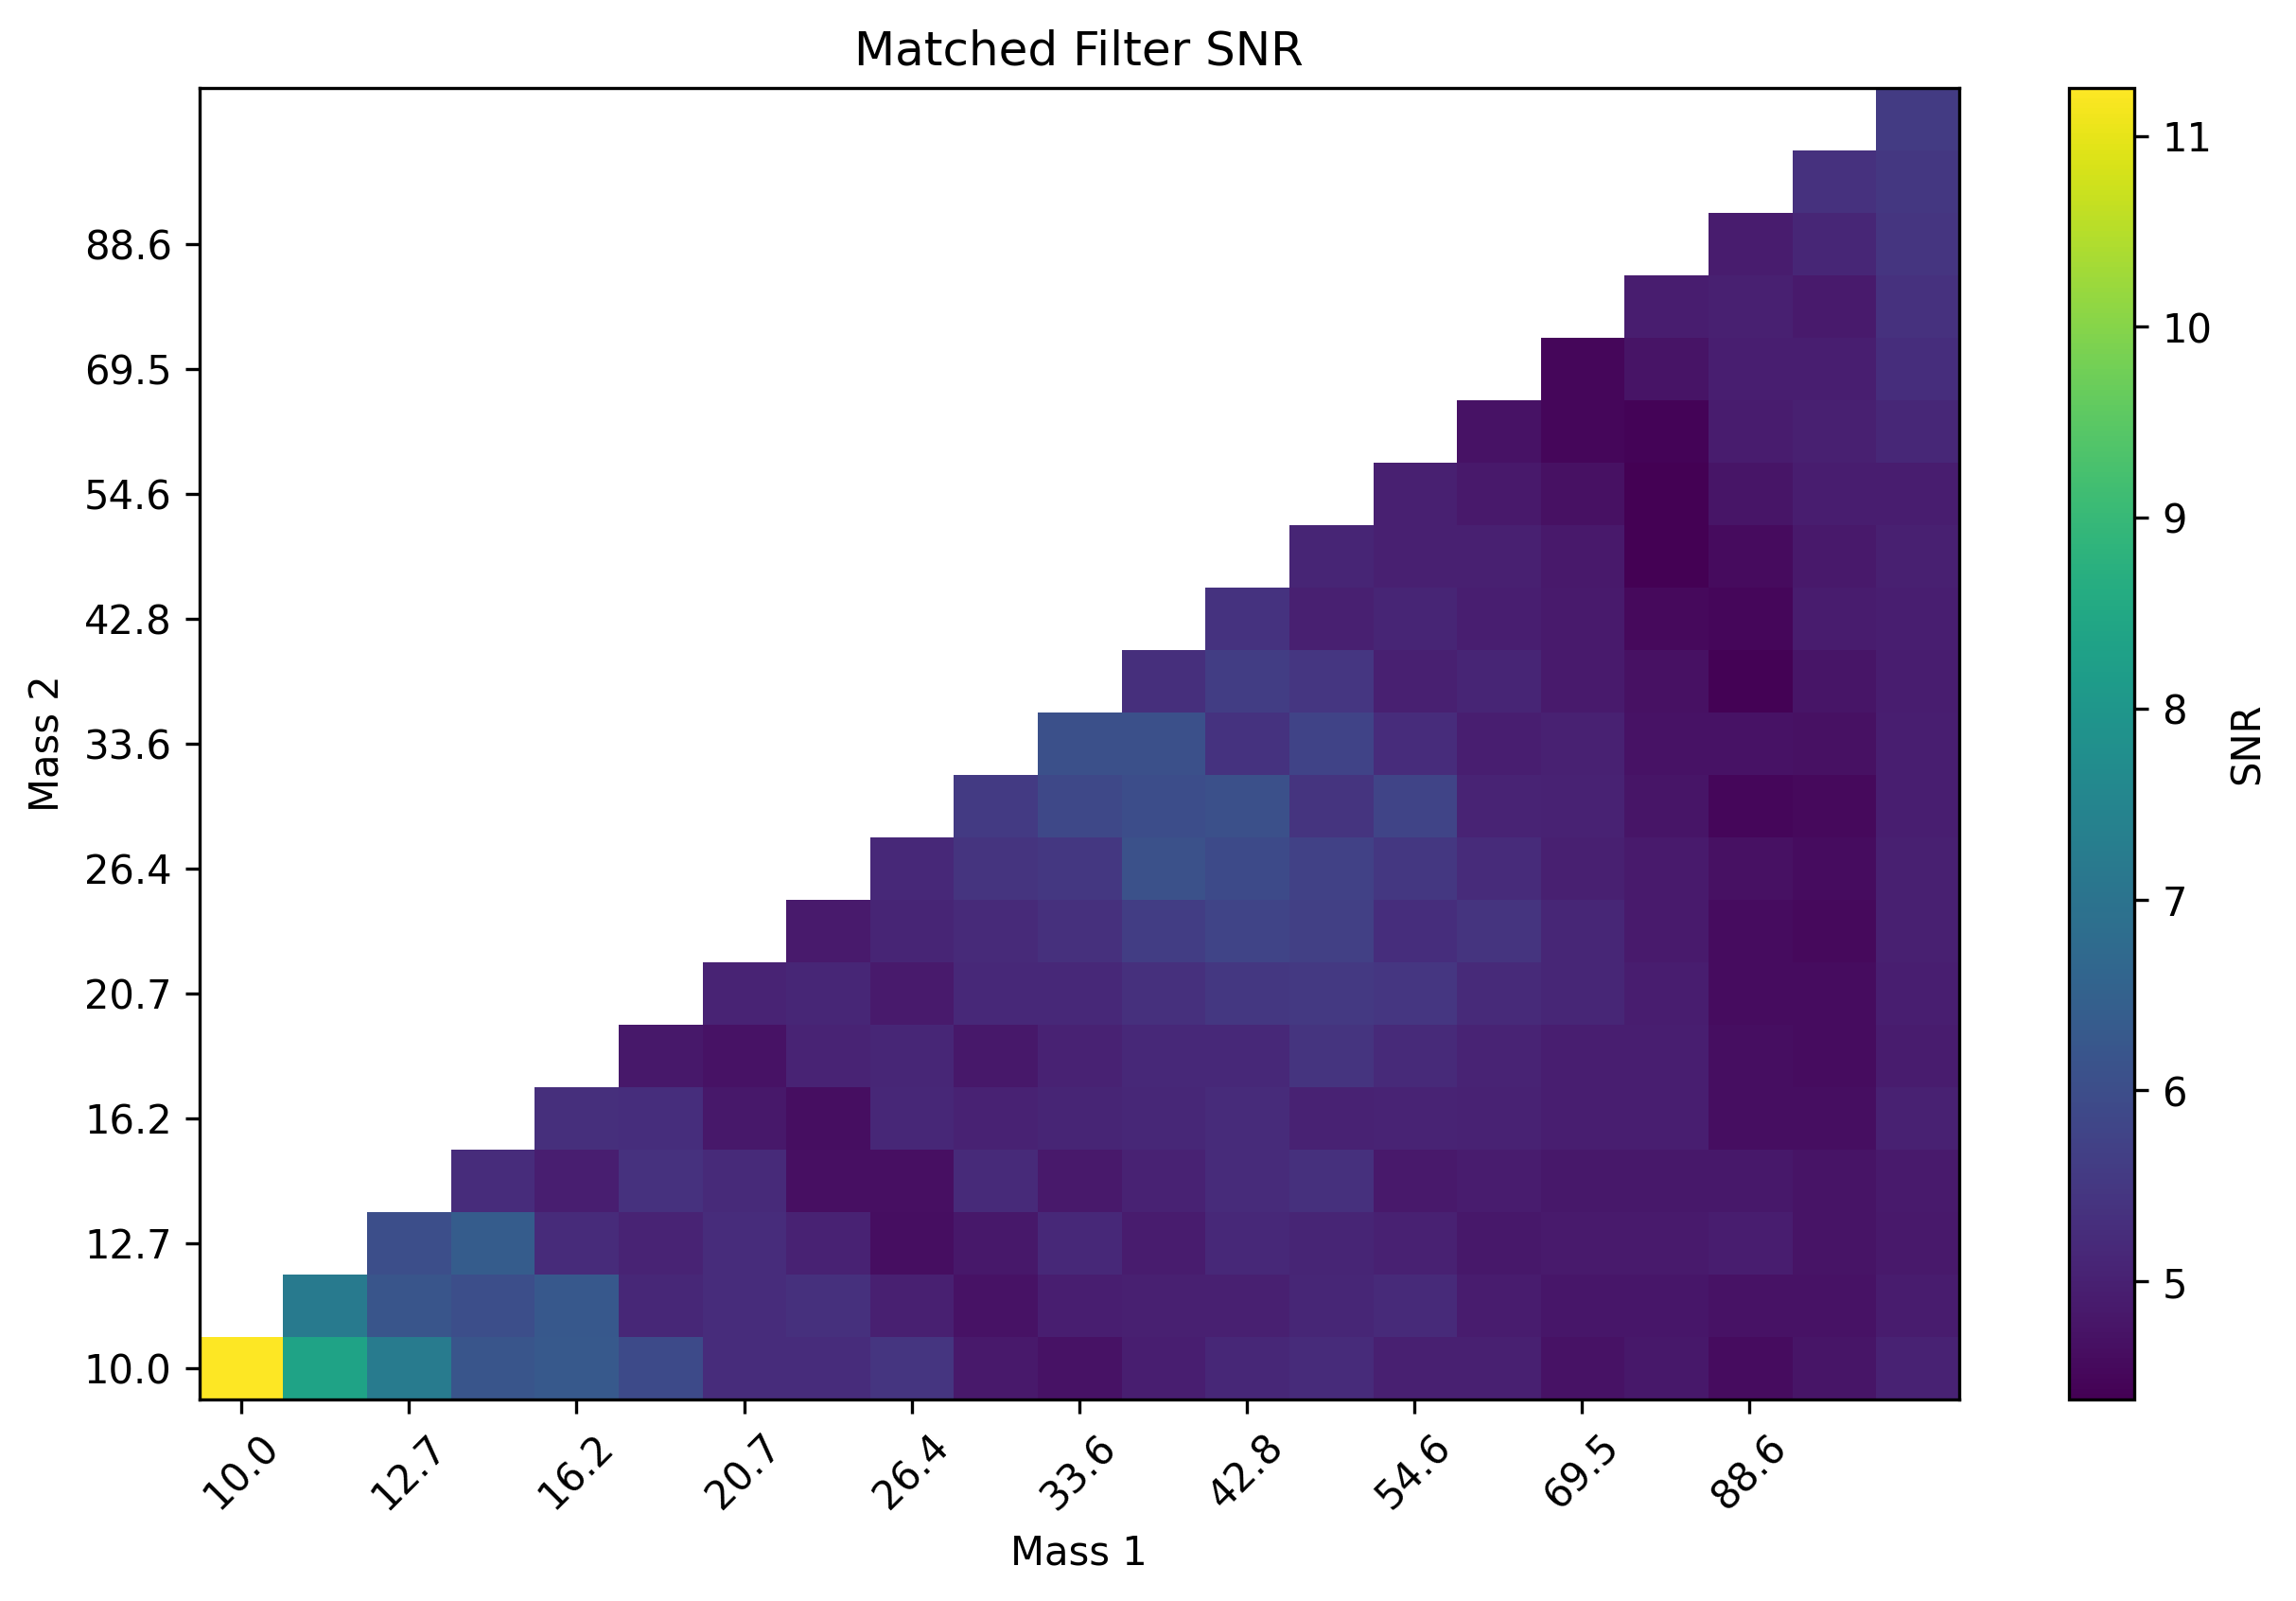
\includegraphics[width=0.8\textwidth]{../plots/mass_space_coarse.png}
    \caption{SNR heatmap from the coarse mass parameter search (10--100 $M_\odot$). The highest SNR corresponds to $M_1 = 10 M_\odot$ and $M_2 = 10 M_\odot$.}
    \label{fig:mass_space_coarse}
\end{figure}

\begin{figure}[H]
    \centering
    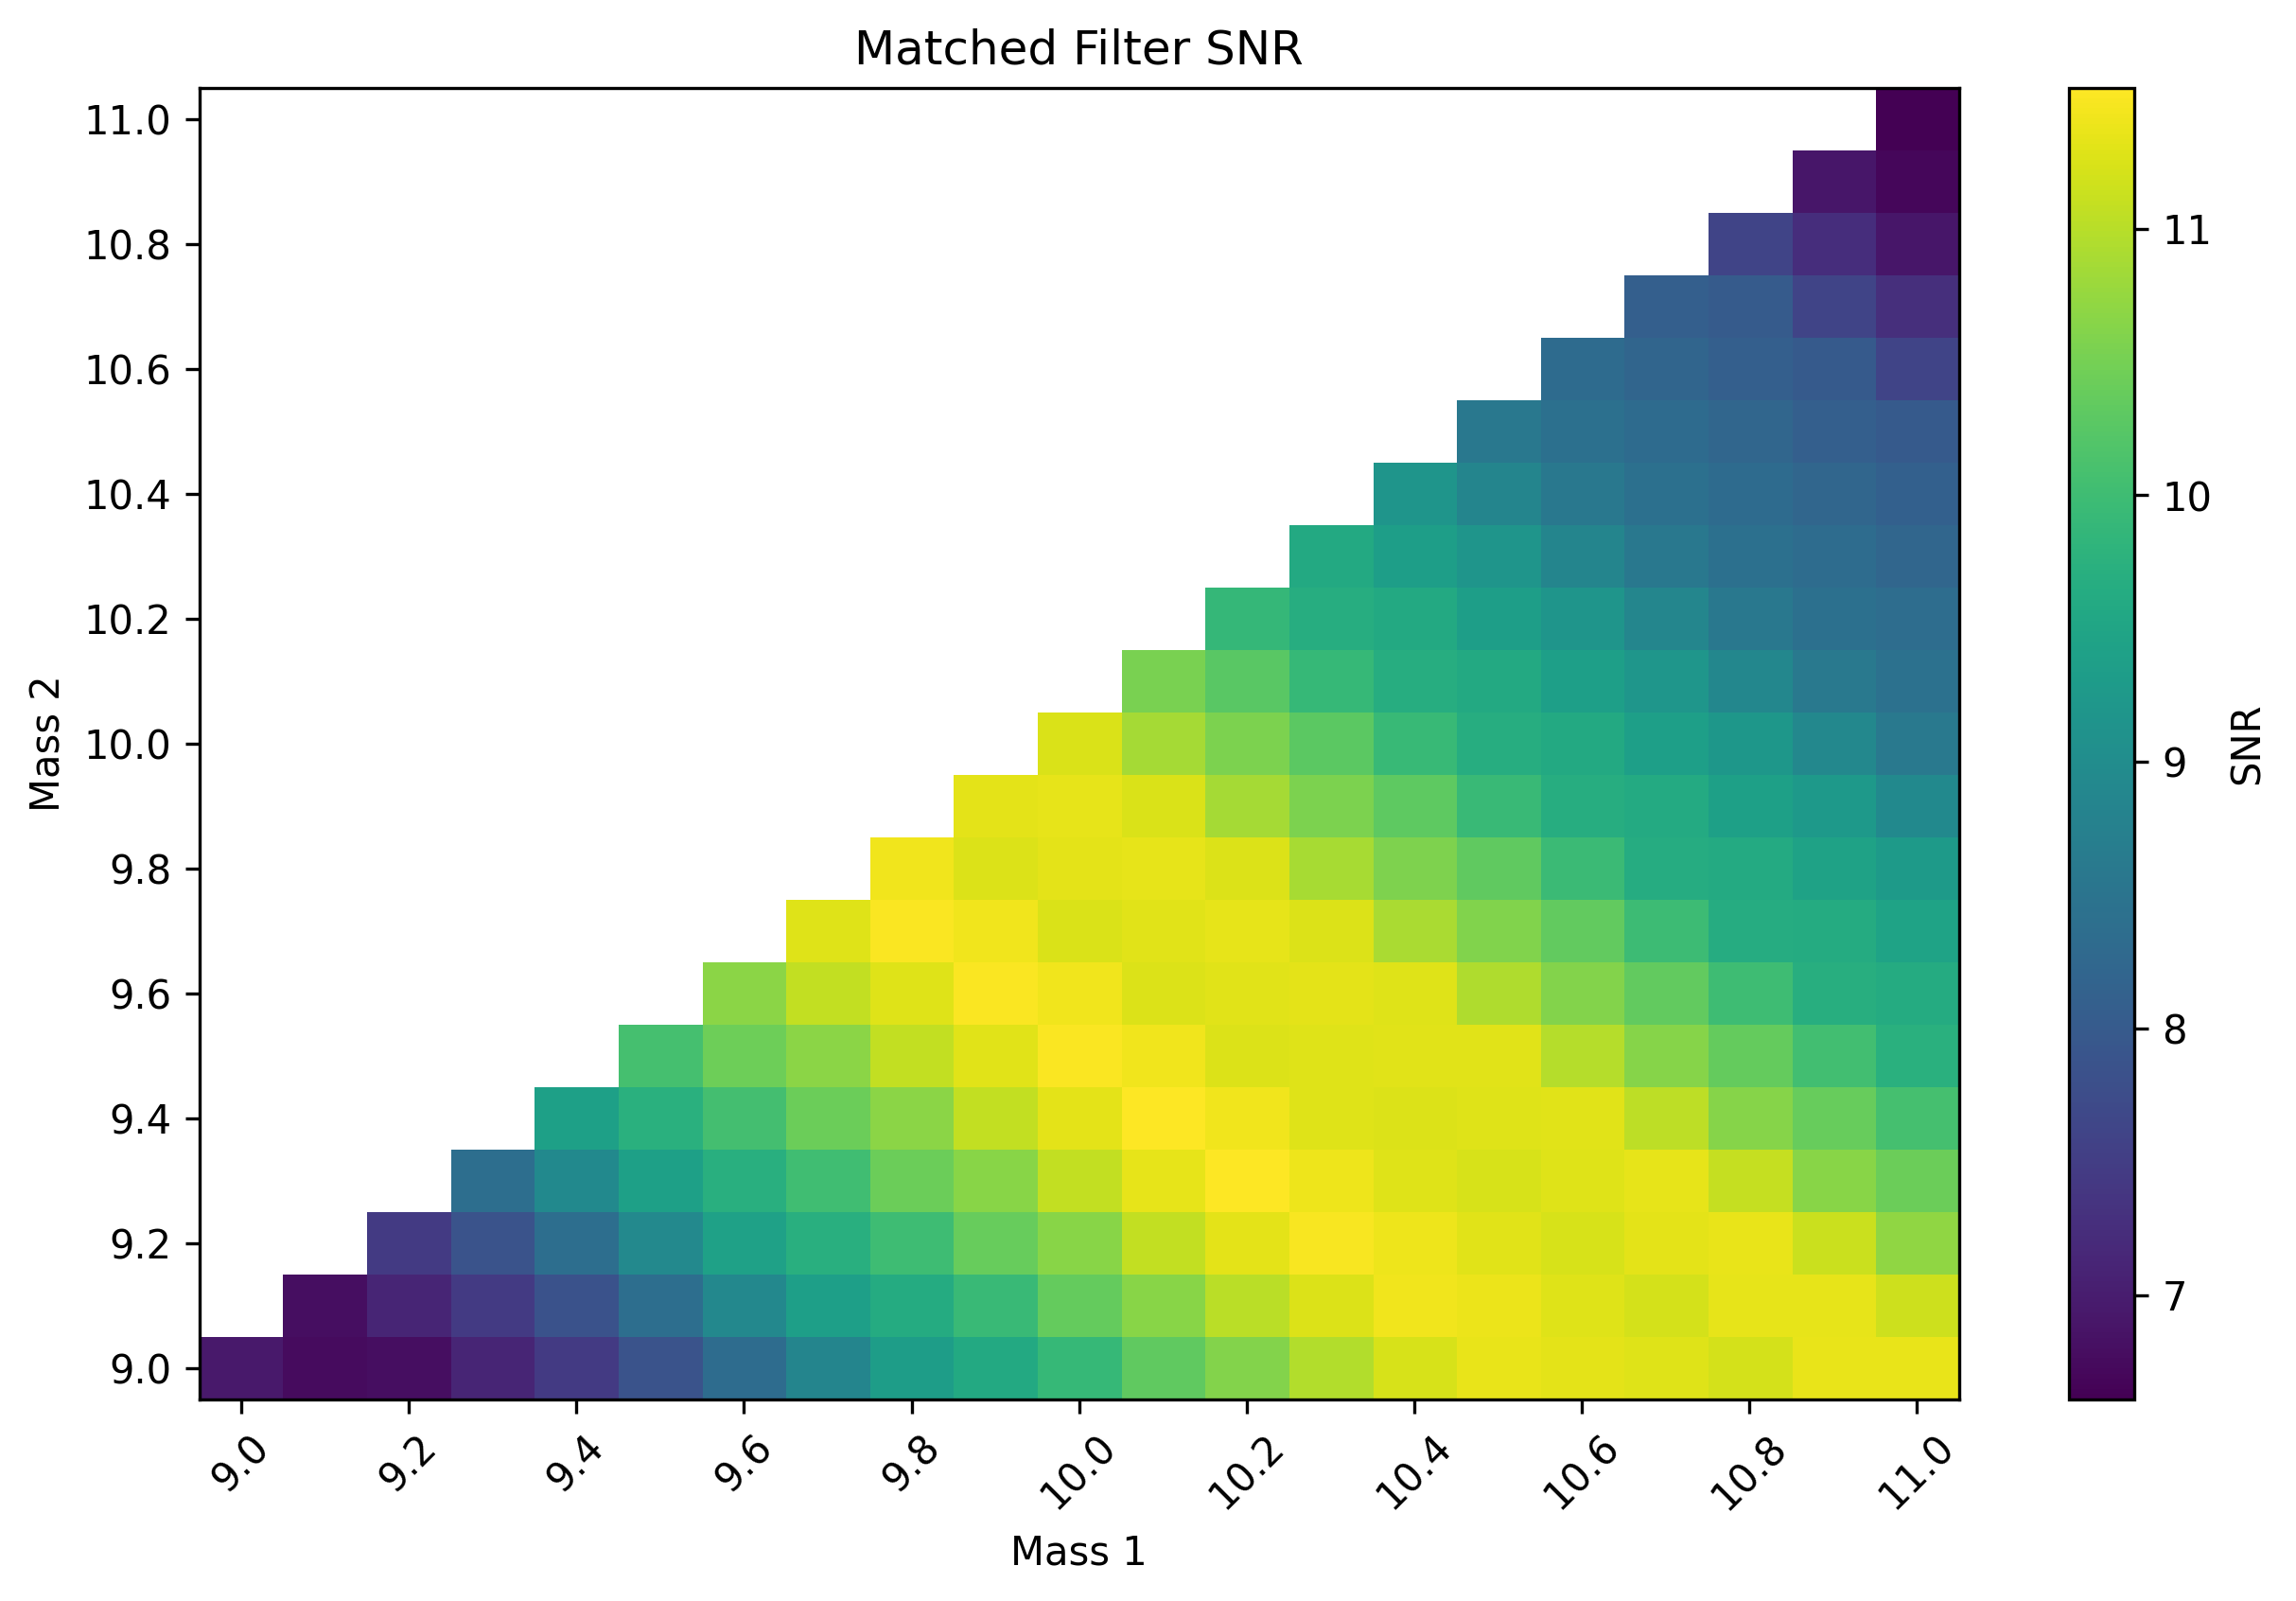
\includegraphics[width=0.8\textwidth]{../plots/mass_space_fine.png}
    \caption{SNR heatmap from the fine mass parameter search (9--11 $M_\odot$). The parameters were refined to $M_1 = 10.1 M_\odot$ and $M_2 = 9.4 M_\odot$.}
    \label{fig:mass_space_fine}
\end{figure}

\begin{figure}[H]
    \centering
    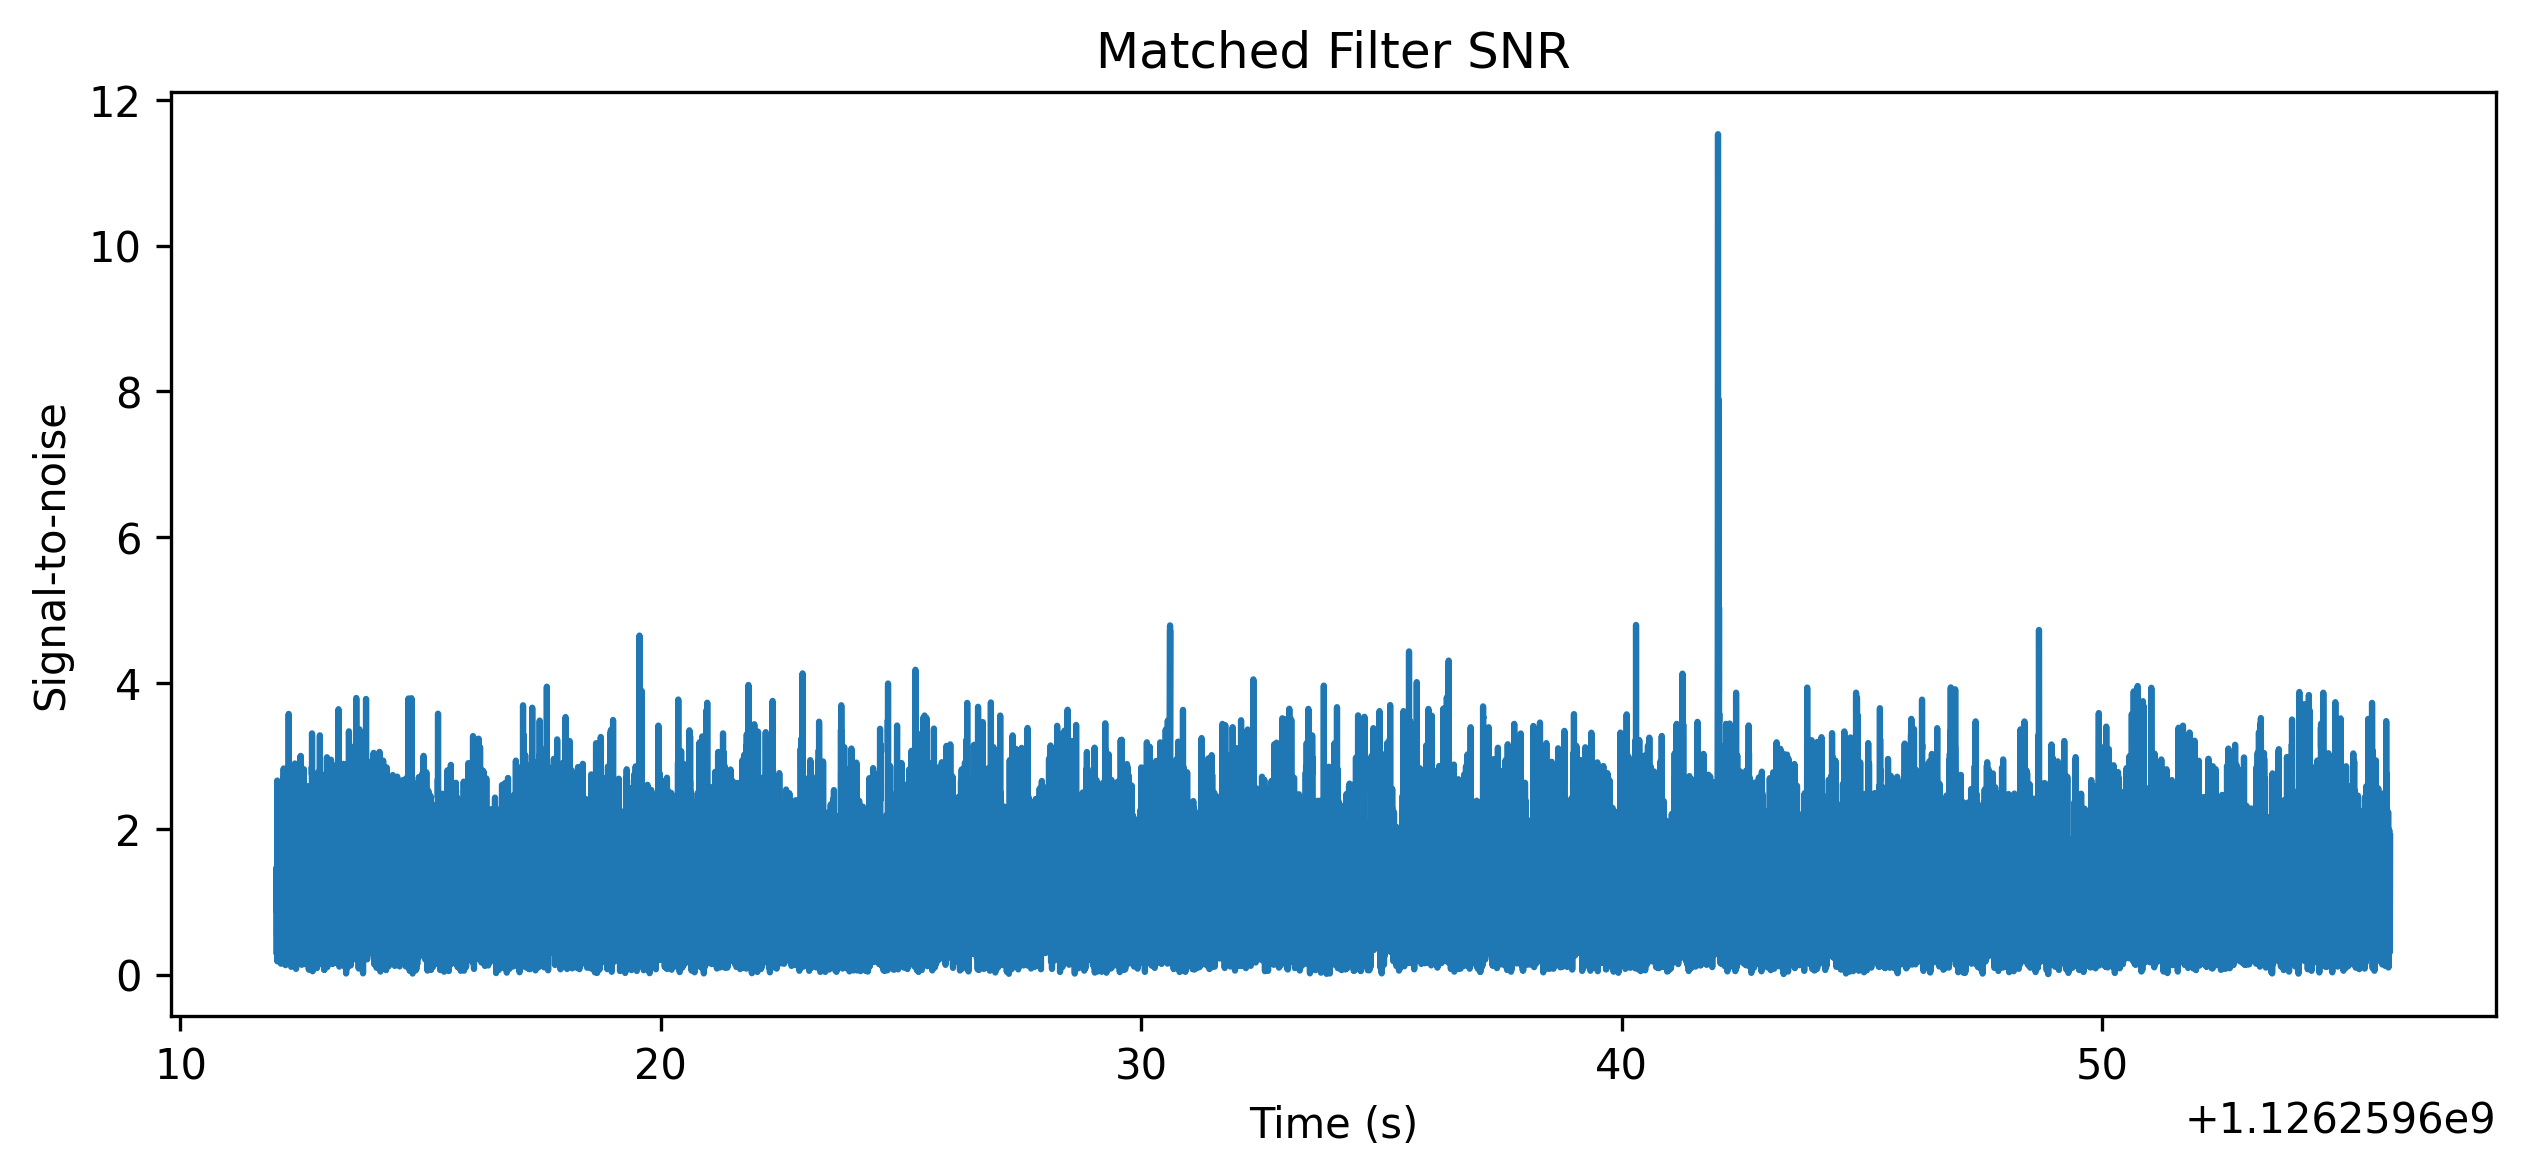
\includegraphics[width=0.8\textwidth]{../plots/matched_filter_snr.png}
    \caption{Matched filter SNR as a function of time shift. The peak SNR corresponds to the gravitational wave signal at 1126259642.0 seconds.}
    \label{fig:matched_filter_snr}
\end{figure}

\begin{figure}[H]
    \centering
    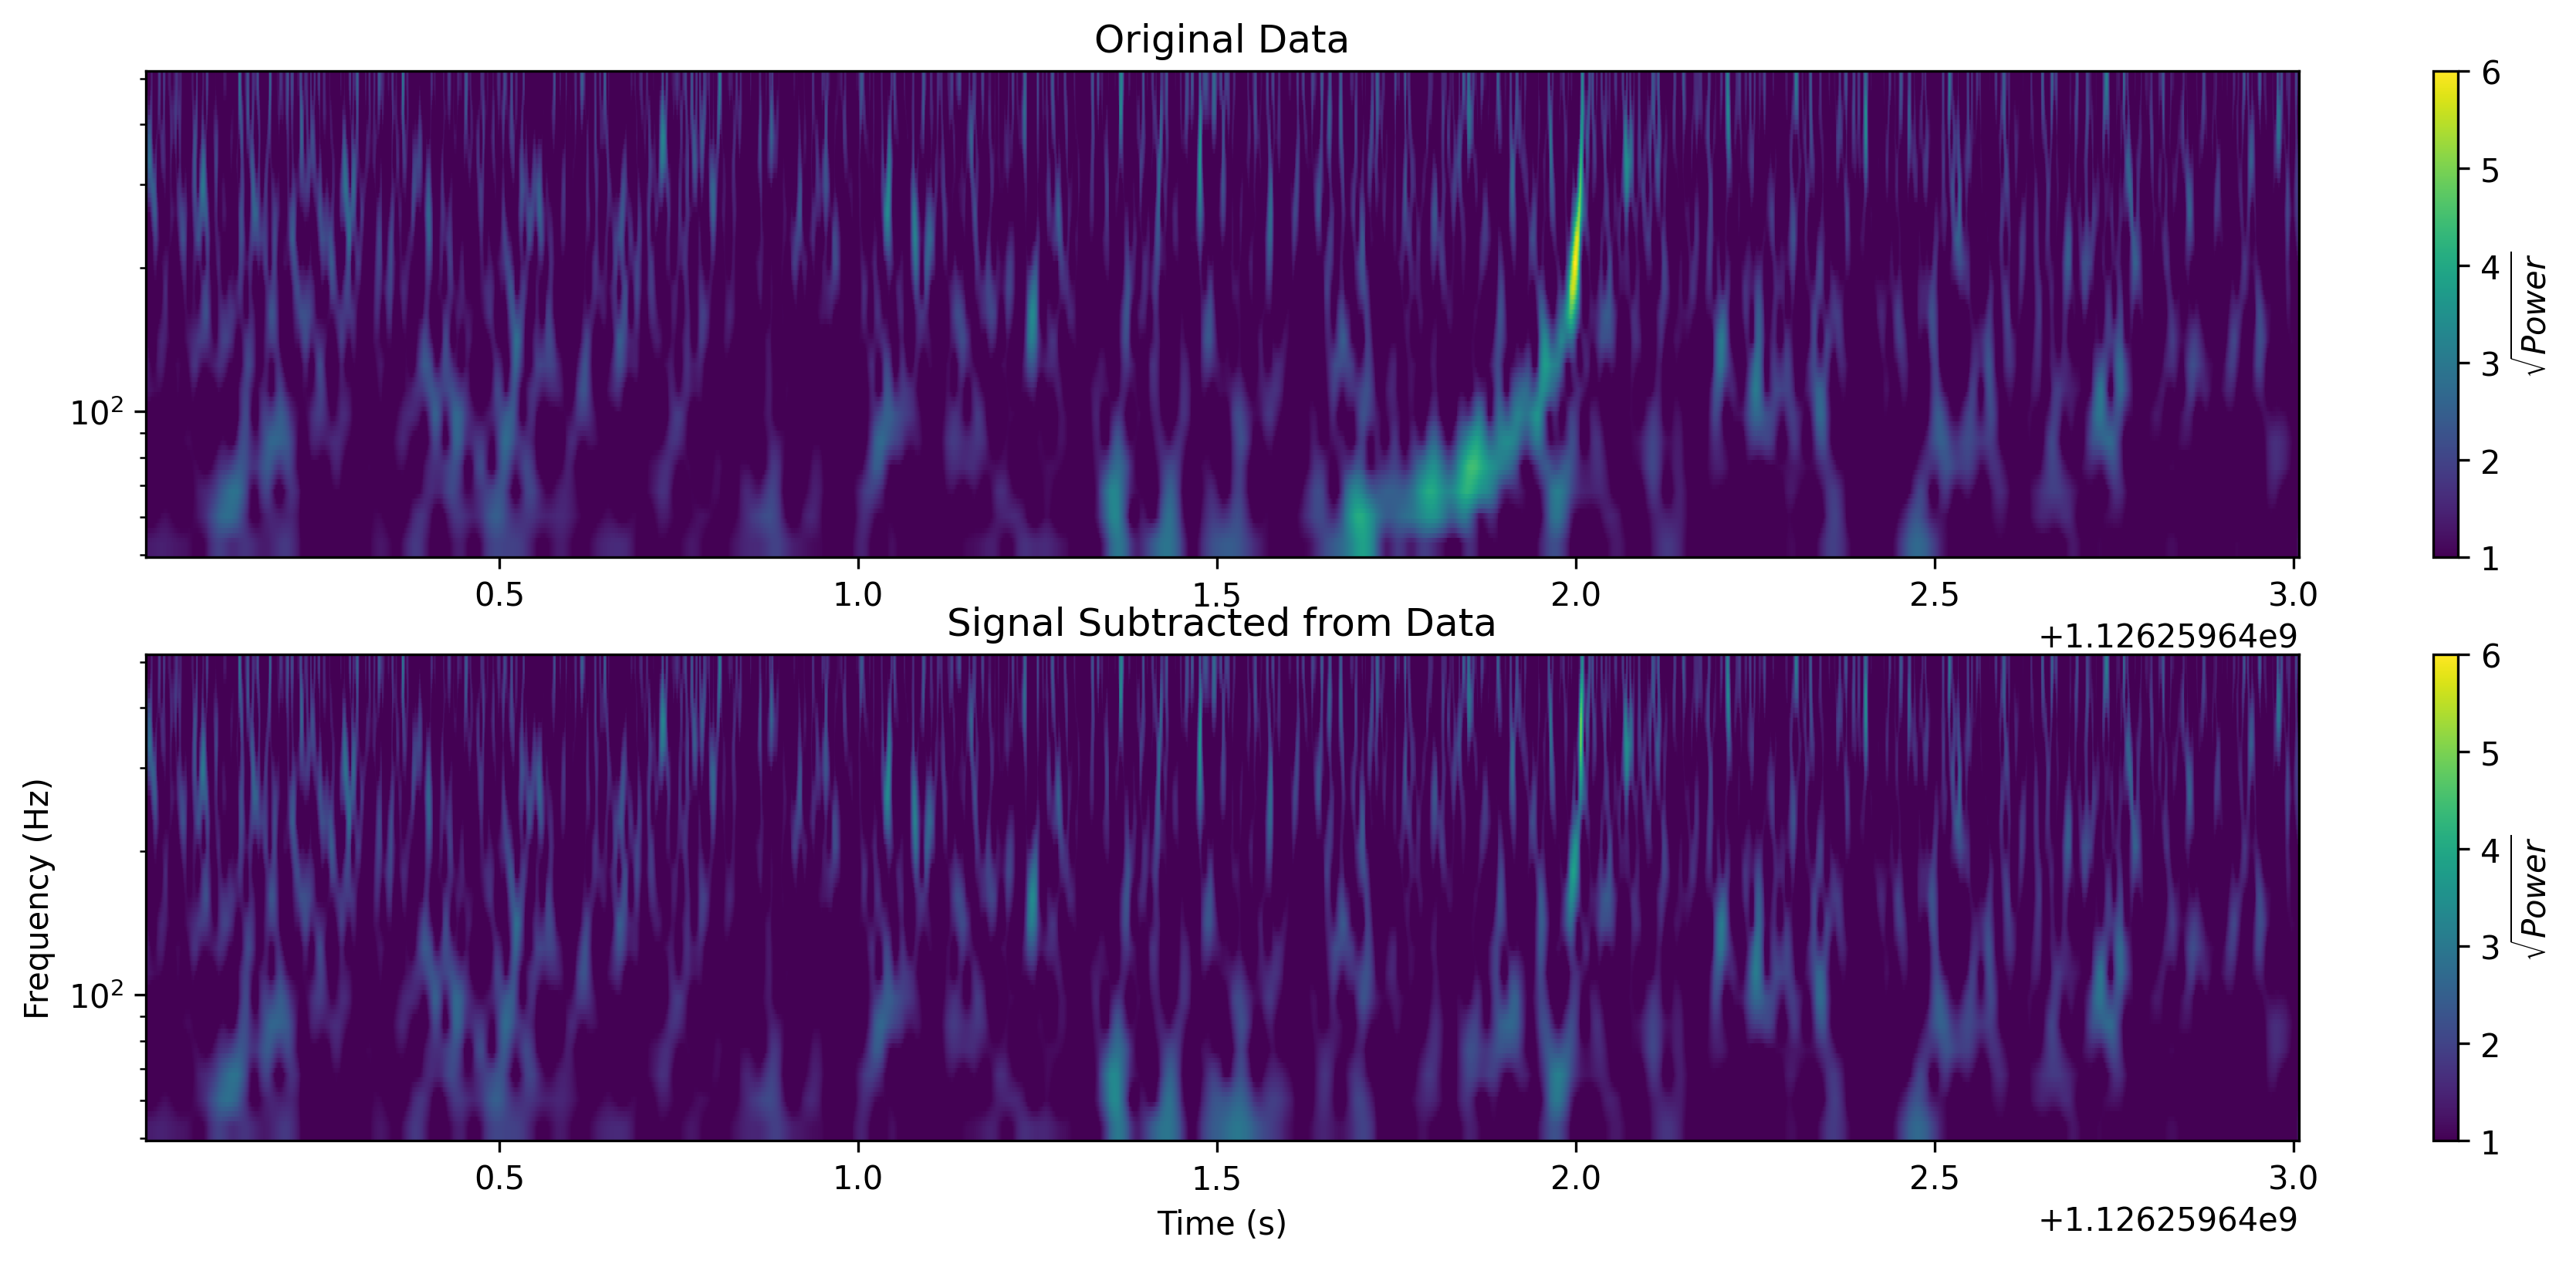
\includegraphics[width=0.8\textwidth]{../plots/subtracted.png}
    \caption{Q-transform of the residual after subtracting the signal from the data. The absence of significant features confirms the extracted signal closely matches the detected gravitational wave.}
    \label{fig:subtracted}
\end{figure}

\begin{figure}[H]
    \centering
    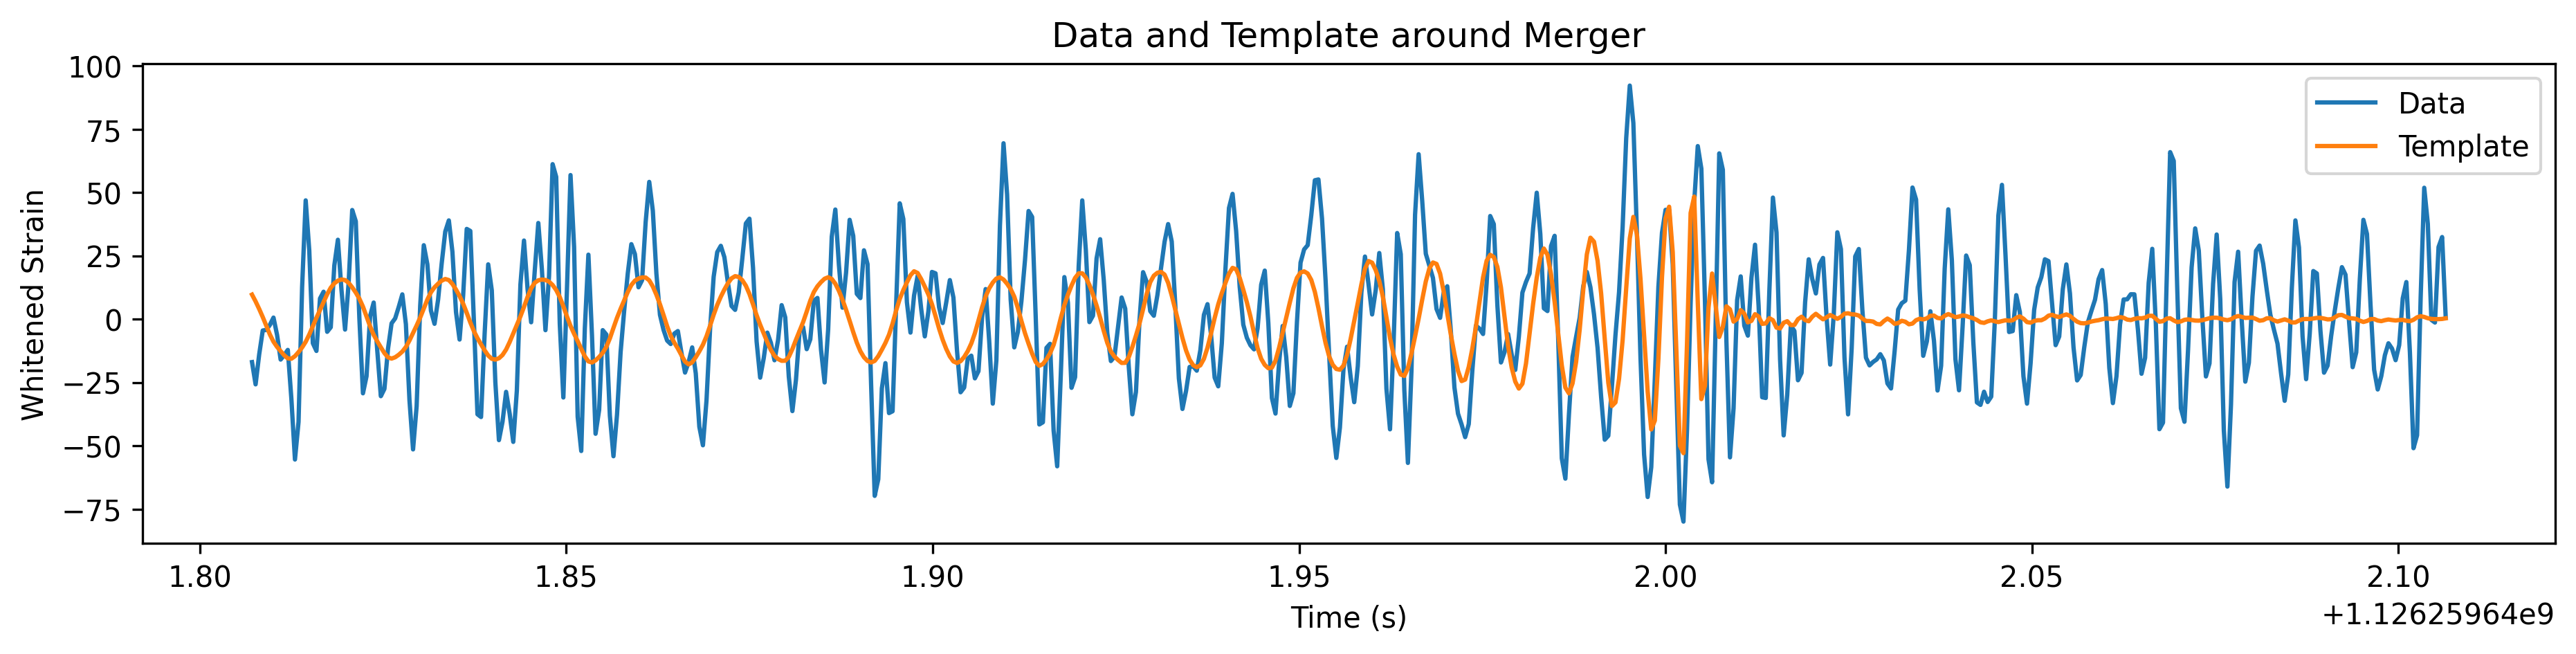
\includegraphics[width=0.8\textwidth]{../plots/overlay_data_template.png}
    \caption{Overlay of the whitened data and best-fit template around the merger event. The excellent agreement highlights the accuracy of the waveform model and parameter estimation.}
    \label{fig:overlay_data_template}
\end{figure}

\section{Discussion}

The results from this analysis strongly indicate that the observed gravitational wave signal is consistent with a binary black hole (BBH) merger. Using matched filtering techniques, the masses of the component black holes were determined to be approximately \( m_1 = 10.1 M_\odot \) and \( m_2 = 9.4 M_\odot \), placing this system within the lower-mass regime for stellar-origin black holes. These values are refined from the coarse parameter space search, demonstrating the importance of iterative template matching for precise parameter estimation.

The matched filter signal-to-noise ratio (SNR) had a sharp peak of height 11.53, indicating a strong correlation between the data and the best-fit waveform template. This high SNR not only confirms the presence of a signal but also validates the accuracy of the mass parameters derived from the analysis. The time-frequency structure of the subtracted Q-transform plot further supports the successful detection and subtraction of the gravitational wave signal, with no significant features remaining in the residual data.

\subsection{Limitations}

While the results are robust, the analysis is limited by the assumptions inherent in the waveform models, such as aligned spins and quasi-circular orbits. Extending the parameter space to include spin-orbit misalignment or eccentric orbits could improve the accuracy of the method. Other models can also be explored in future work so that NSBH and BNS systems are also detected.

\printbibliography[heading=bibintoc,title={References}]

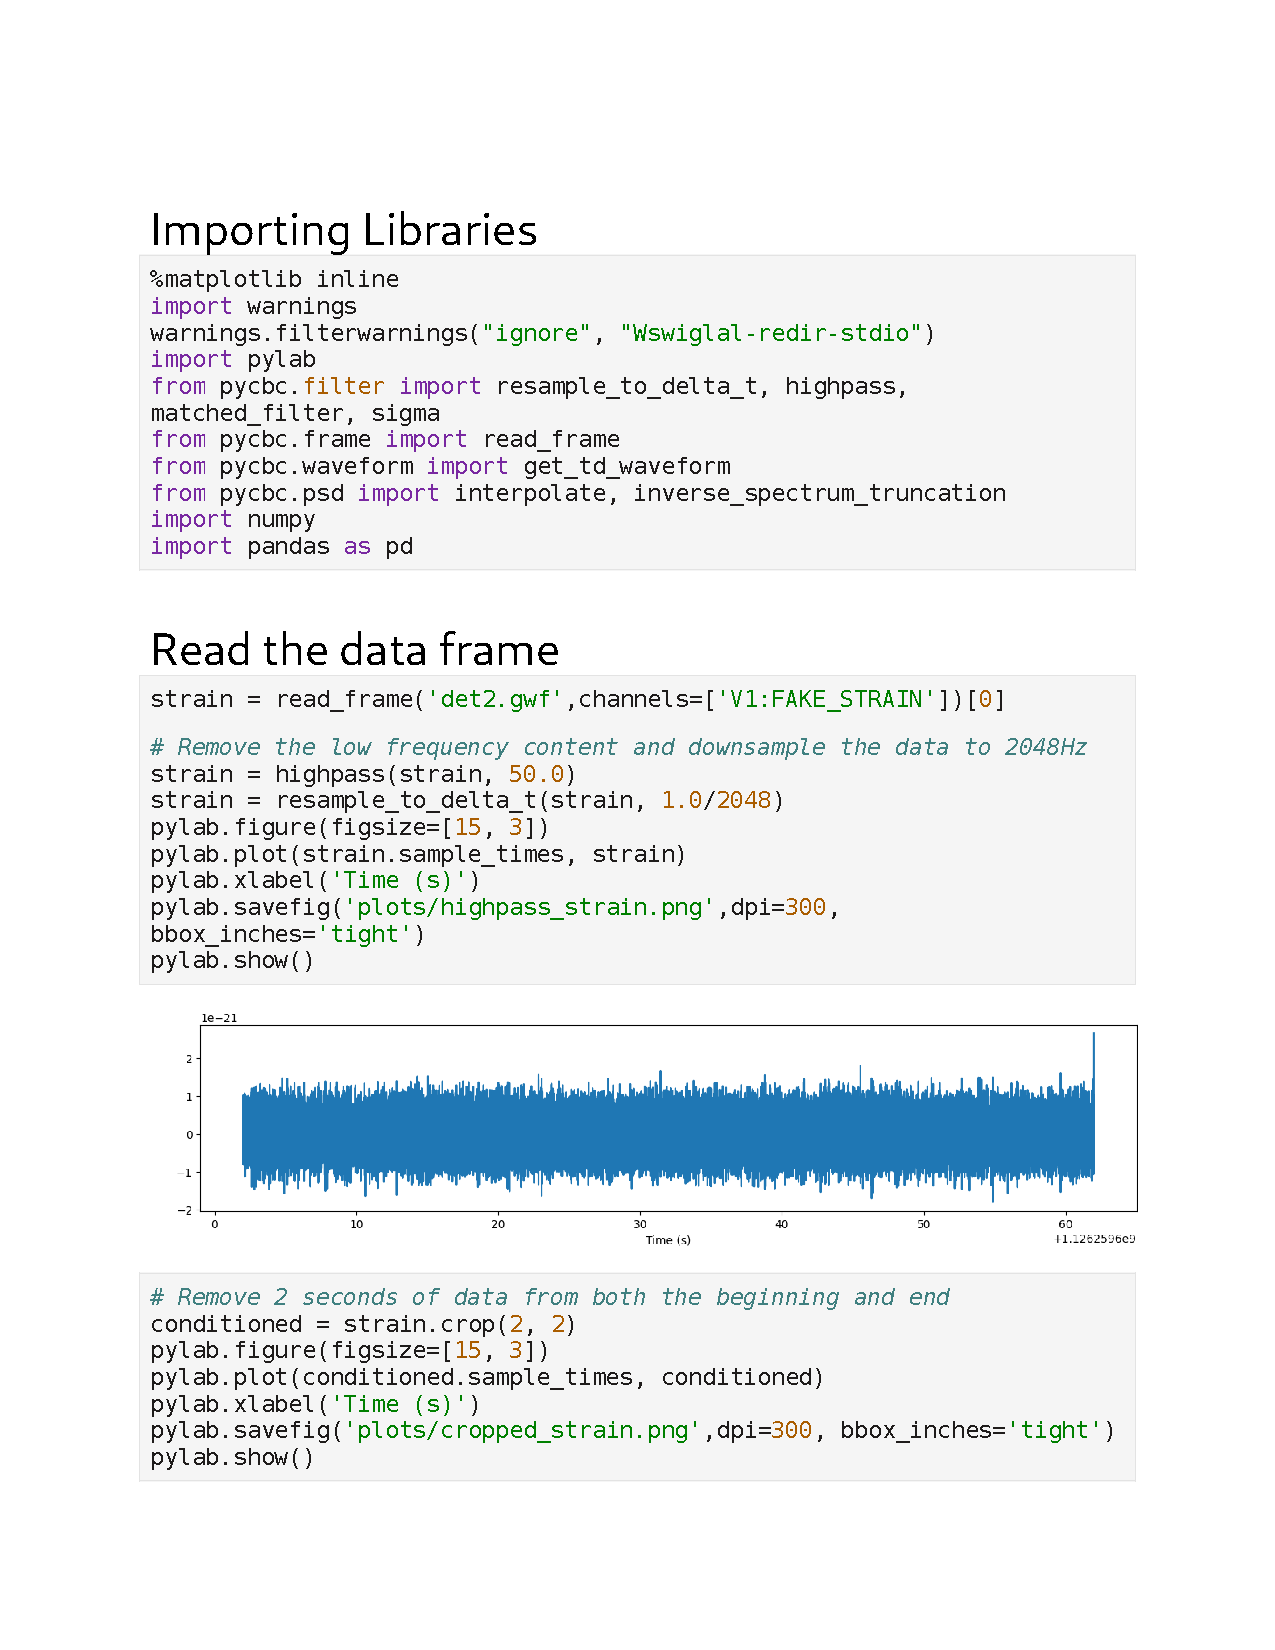
\includepdf[
    pages=-,
    pagecommand={\pagestyle{headings}},  
    addtotoc={1,section,1,Appendix - Code,sec:code}]
{../match_filtering_code.pdf}

\end{document}
